\documentclass{standalone}
\usepackage[latin1]{inputenc}
\usepackage{tikz}
\usetikzlibrary{shapes, arrows}
% Define block styles
\tikzstyle{decision} = [diamond, draw, fill=blue!20, text width=4.5em, 
    text badly centered, node distance=3cm, inner sep=0pt]
\tikzstyle{block} = [rectangle, draw, fill=blue!20, text width=5em, 
    text centered, rounded corners, minimum height=4em]
\tikzstyle{line} = [draw, -latex']
\tikzstyle{cloud} = [draw, ellipse,fill=red!20, node distance=3cm,
    minimum height=2em]
\tikzstyle{io} = [trapezium, trapezium left angle=70, trapezium right angle=110, 
    minimum height=1cm, text centered, draw=black, fill=blue!30]

\begin{document}
    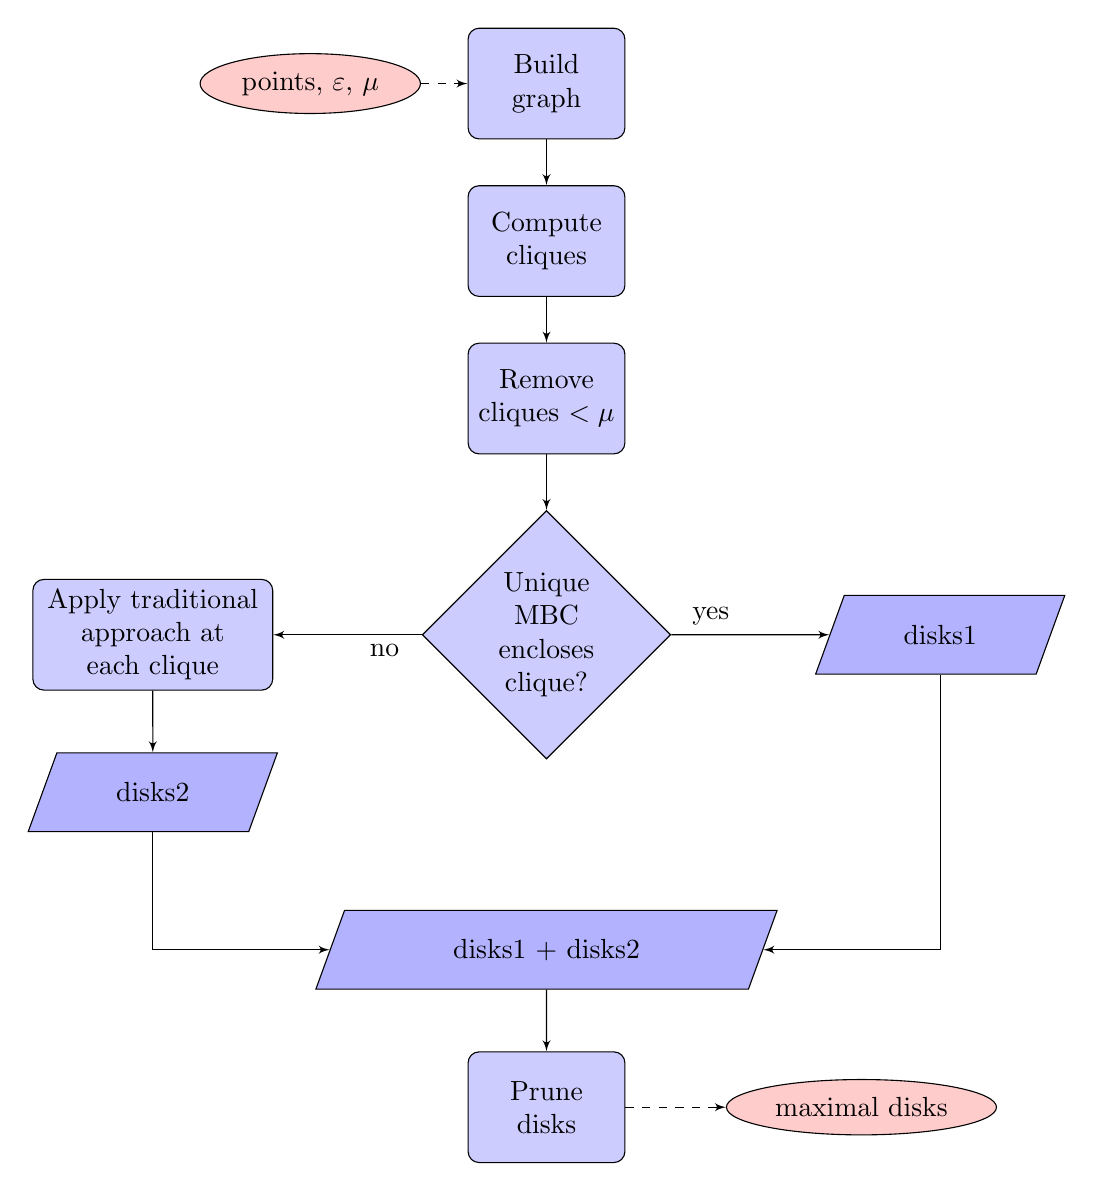
\begin{tikzpicture}[node distance = 2cm, auto]
        % Place nodes
        \node [block] (graph) {Build graph};
        \node [cloud, left of=graph] (input) {points, $\varepsilon$, $\mu$};
        \node [block, below of=graph] (cliques) {Compute cliques};
        \node [block, below of=cliques] (filter) {Remove cliques $< \mu$};
        \node [decision, below of=filter] (decide) {Unique MBC encloses clique?};
        \node [io, right of=decide, node distance=5cm] (disks1) {disks1};
        \node [block, left of=decide, node distance=5cm, text width=8em] (traditional) {Apply traditional approach at each clique};
        \node [io, below of=traditional] (disks2) {disks2};
        \node [io, below of=decide, node distance=4cm] (disks) {disks1 + disks2};
        \node [block, below of=disks] (prune) {Prune disks};
        \node [cloud, right of=prune, node distance=4cm] (maximals) {maximal disks};
        % Draw edges
        \path [line,dashed] (input) -- (graph);
        \path [line] (graph) -- (cliques);
        \path [line] (cliques) -- (filter);
        \path [line] (filter) -- (decide);
        \path [line] (decide) -- node [near start] {yes} (disks1);
        \path [line] (decide) -- node [near start] {no}  (traditional);
        \path [line] (traditional) -- (disks2);
        \path [line] (disks1) |- (disks);
        \path [line] (disks2) |- (disks);
        \path [line] (disks) -- (prune);
        \path [line,dashed] (prune) -- (maximals);
    \end{tikzpicture}
\end{document}
